\documentclass[aspectratio=169,11pt]{beamer}
\usepackage[utf8]{inputenc}
\DeclareUnicodeCharacter{21D2}{$\Rightarrow$}
\DeclareUnicodeCharacter{21A6}{$\mapsto$}
\DeclareUnicodeCharacter{2080}{$_0$}
\DeclareUnicodeCharacter{03BC}{$\mu$}
\DeclareUnicodeCharacter{03B5}{$\varepsilon$}
\DeclareUnicodeCharacter{2264}{$\leq$}
\DeclareUnicodeCharacter{2265}{$\geq$}
\DeclareUnicodeCharacter{2260}{$\neq$}
\DeclareUnicodeCharacter{2205}{$\emptyset$}
\DeclareUnicodeCharacter{2192}{$\to$}
\DeclareUnicodeCharacter{211D}{$\mathbb{R}$}
\DeclareUnicodeCharacter{2264}{$\leq$}
\DeclareUnicodeCharacter{22C6}{$\star$}
\DeclareUnicodeCharacter{2217}{$*$}
\DeclareUnicodeCharacter{2AAF}{$\preceq$}
\usepackage[T1]{fontenc}
\usepackage[english]{babel}
\usepackage{amsmath,amssymb}
\usepackage{booktabs}
\usepackage{graphicx}
\usepackage{listings}
\usetheme{default}
\usecolortheme{seahorse}
\setbeamertemplate{navigation symbols}{}
\setbeamertemplate{footline}[frame number]
\setbeamerfont{frametitle}{size=\large}

\lstdefinelanguage{Lean}{
  morekeywords={theorem,lemma,def,noncomputable,by,intro,apply,exact,have,rw,simp,only,
    linarith,nlinarith,omega,show,fun,let,if,then,else,Prop,Type,refine,constructor,
    rintro,field_simp,at,ring,StrictMonoOn,max},
  sensitive=true,
  morecomment=[l]{--},
  morecomment=[s]{/-}{-/},
}
\lstset{
  language=Lean,
  basicstyle=\ttfamily\scriptsize,
  keywordstyle=\color{blue!70!black}\bfseries,
  commentstyle=\color{gray},
  columns=fullflexible,
  keepspaces=true,
  breaklines=true,
  extendedchars=true,
  inputencoding=utf8,
  literate=
    {∀}{{$\forall$}}1 {∃}{{$\exists$}}1 {ℝ}{{$\mathbb{R}$}}1 {→}{{$\to$}}1 {↔}{{$\leftrightarrow$}}1
    {∈}{{$\in$}}1 {≤}{{$\leq$}}1 {≥}{{$\geq$}}1 {≠}{{$\neq$}}1 {⟨}{{$\langle$}}1 {⟩}{{$\rangle$}}1
    {₀}{{$_0$}}1 {¬}{{$\neg$}}1 {∧}{{$\wedge$}}1 {·}{{$\cdot$}}1 {⇒}{{$\Rightarrow$}}1
    {←}{{$\leftarrow$}}1 {⋆}{{$\star$}}1 {∗}{{$*$}}1 {⁻¹}{{$^{-1}$}}2
}

\title{Ide \& Talamàs (2025)}
\subtitle{\emph{Artificial Intelligence in the Knowledge Economy} --- who gains, on which condition, and what Lean checks}
\author{Manuel Arriola}
\date{Repository 5 \textperiodcentered{} Week of September 14 -- 19, 2026}

\begin{document}

%================= PORTADA =============================================
\begin{frame}[plain]
  \titlepage
  \begin{center}\small
    \texttt{github.com/Arriola123456/ai-05-ide}\\[2pt]
    \footnotesize Version read: arXiv 2312.05481\textbf{v11} (24 Feb 2025, 35 pp., pinned by SHA-256 in \texttt{lean/});
    v12 (May 2025, 39 pp.) is the course PDF, same Propositions 1--6. Backup slides after slide 14.
  \end{center}
\end{frame}

%================= 1. EL PAPER Y EL PROBLEMA =========================
\begin{frame}{1 \textperiodcentered{} The paper and the agent's problem}
  \footnotesize
  \textbf{Question.} Modern AI does non-codifiable cognitive work and, unlike a human expert, can be copied across
  compute. Who gains when it enters an economy in which people organise into \emph{workers} (routine problems) and
  \emph{solvers} (exceptions)? The answer separates two dimensions: \textbf{capability} $z_{AI}$ and \textbf{autonomy}.

  \smallskip
  \textbf{Pre-AI economy (Section 3.1, p.\ 10).} Knowledge $z\in[0,1]$, density $g>0$. A problem has difficulty
  $x\sim U[0,1]$; it is solved (one unit of output) if the knowledge applied to it is $\ge x$.
  \begin{itemize}
    \item One-layer firm: an independent producer, expected output $z$.
    \item Two-layer firm: one solver $s$ and workers $z\le s$; a stuck worker asks the solver at time cost $h\in(0,1)$.
      The solver's time is exhausted by
      \[
        h\,n(z)\,(1-z)=1 \quad\Longleftrightarrow\quad n(z)=\frac{1}{h(1-z)},\qquad \text{team output } n(z)\,s .
      \]
  \end{itemize}
  \textbf{AI (p.\ 11).} One unit of compute (rental $r$) $\mapsto$ one agent of knowledge $z_{AI}\in[0,1)$, a perfect
  substitute for a human with that knowledge. \emph{Autonomous:} independent producer, worker or solver.
  \emph{Non-autonomous} (Section 6): solver only. Compute is abundant relative to human time.
\end{frame}

\begin{frame}{1 \textperiodcentered{} The five firms and the equilibrium (p.\ 12--13)}
  \footnotesize
  Taking the wage schedule $w(\cdot)$ and $r$ as given, a firm chooses the most profitable structure:
  \begin{gather*}
    \Pi_1 = z-w(z)\ \text{ or }\ z_{AI}-r,\qquad
    \Pi_2^{tA}(z)=n(z)[z_{AI}-w(z)]-r,\\
    \Pi_2^{bA}(s)=n(z_{AI})[s-r]-w(s),\qquad
    \Pi_2^{nA}(s,z)=n(z)[s-w(z)]-w(s).
  \end{gather*}
  Each profit is expected output minus the cost of the resources used (top-automated $tA$: humans under an AI solver;
  bottom-automated $bA$: AI workers under a human solver; $nA$: humans only). No AI--AI firm: an AI solver knows what an
  AI worker knows.

  \smallskip
  \textbf{Competitive equilibrium (Definition, p.\ 13).} Compute allocation $(\mu_i,\mu_w,\mu_s)$, occupations
  $(I,W_p,W_a,S_p,S_a)$, a matching $m:W_p\to S_p$ with solver time clearing,
  $\int_Y h(1-u)\,dG(u)=\int_{m(Y)}dG(u)$, wages $w$ and rental $r$ such that firms optimise at zero profit and markets
  clear. Efficient (First Welfare Theorem) $\Rightarrow$ wages are marginal products.

  \smallskip
  \textbf{Two maintained assumptions.} $h<h_0$: no independent producers before AI (p.\ 18). Compute abundant relative
  to time: some agents \emph{must} produce independently (footnote 14) $\Rightarrow$ $r^*=z_{AI}$ with autonomy,
  $r^\star=0$ without.
\end{frame}

%================= 2. RESULTADO PRINCIPAL ============================
\begin{frame}{2 \textperiodcentered{} Prices and wages with autonomous AI (Proposition 2, p.\ 19)}
  \footnotesize
  Unique, efficient equilibrium; stratification $W^*\preceq\{z_{AI}\}\preceq S^*$; positive assortative matching.
  AI is always an independent producer; also a \textbf{worker} if $z_{AI}\in W$ (\emph{basic} AI), a \textbf{solver}
  if $z_{AI}\in S$ (\emph{advanced} AI). Prices:
  \[
    r^*=z_{AI},\qquad
    w^*(z)=z_{AI}\Big(1-\tfrac{1}{n(z)}\Big)\ (z\in W^*_a),\qquad
    w^*(z)=n(z_{AI})\,(z-z_{AI})\ (z\in S^*_a),\qquad w^*(z_{AI})=z_{AI}.
  \]
  All three come from zero profit: $z_{AI}-r=0$; $n(z)[z_{AI}-w]-z_{AI}=0$; $n(z_{AI})[s-z_{AI}]-w=0$.
  The AI solver keeps $z_{AI}/n(z)$ of each assisted worker's output; a human supervising AI workers keeps the whole
  surplus $s-z_{AI}$ over $n(z_{AI})$ agents. The person with $z=z_{AI}$ \emph{always loses}: $w^*(z_{AI})=z_{AI}<w(z_{AI})$
  because pre-AI $w(z)>z$ for all $z$ when $h<h_0$ (Proposition 1).
\end{frame}

\begin{frame}{2 \textperiodcentered{} The main result: Propositions 5 and 6, with all their conditions}
  \footnotesize
  $B=\{z\le z_{AI}: w^*(z)>w(z)\}=[0,z_b)$, \ $T=\{z\ge z_{AI}: w^*(z)>w(z)\}=(z_t,1]$ (winners sit at the extremes).

  \textbf{Proposition 5 (p.\ 24, autonomous AI).} There are winners at the bottom \emph{if AI is good enough}:
  $B\ne\emptyset\iff z_{AI}>\bar z_{AI}$, with $\bar z_{AI}\in\operatorname{int}W$. There are \emph{always} winners at the top:
  $T\ne\emptyset$ for all $z_{AI}\in[0,1)$.

  \textbf{Proposition 6 (p.\ 27, non-autonomous AI).} $r^\star=0$. AI is used iff $z_{AI}>w(0)$, and then only by the least
  knowledgeable. In any case: (1) output is strictly higher with autonomous AI; (2) non-autonomous AI creates losers;
  (3) near $z=0$: $w^\star\ge\max\{w,w^*\}$, strictly if $z_{AI}>w(0)$; (4) near $z=1$: $w^\star\le w^*$.

  \smallskip
  \textbf{Conditions, spelled out.}
  \begin{enumerate}\setlength{\itemsep}{0pt}
    \item $g$ continuous and $>0$; $x\sim U[0,1]$ without loss (fn.\ 10); at most two layers.
    \item $h\in(0,1)$ and $h<h_0$ (no independent producers pre-AI); \emph{top always gains} also needs $z_{AI}<1$ ---
      a superintelligent AI makes the most knowledgeable lose (fn.\ 19).
    \item Compute abundant relative to time (fn.\ 14), the same compute in both regimes.
    \item An AI agent is a perfect substitute for a human of knowledge $z_{AI}$ (autonomous case); one $z_{AI}$ for all agents.
    \item Zero profits, wages = marginal products: the equilibrium is the planner's LP (used in the numerics).
  \end{enumerate}
\end{frame}

\begin{frame}{2 \textperiodcentered{} Two dimensions, not one: capability decides \emph{whether}, autonomy decides \emph{how much}}
  \footnotesize
  \begin{center}\scriptsize
  \begin{tabular}{@{}lll@{}}
    \toprule
     & \textbf{Autonomous} (co-worker + co-pilot) & \textbf{Non-autonomous} (co-pilot only)\\
    \midrule
    Rental rate & $r^*=z_{AI}$ & $r^\star=0$ (idle compute)\\
    Bottom gains iff & $z_{AI}>\bar z_{AI}\in\operatorname{int}W$ (Prop.\ 5) & $z_{AI}>w(0)$ (Prop.\ 6)\\
    Bottom's wage when AI-assisted & $z_{AI}\,(1-1/n(z))$ & $z_{AI}$ (whole team output)\\
    Top & always gains (Prop.\ 5) & may lose; $w^\star\le w^*$ at the top (6.2, 6.4)\\
    Output & higher (Prop.\ 6.1) & lower\\
    \bottomrule
  \end{tabular}
  \end{center}
  \smallskip
  The \textbf{condition for winners at the bottom is about capability in both regimes} --- a threshold on $z_{AI}$.
  What autonomy changes is the threshold ($w(0)<\bar z_{AI}$), the size of the bottom's gain, the fate of the top and
  total output. The gloss ``the distributional effect is driven by autonomy, not capability'' keeps the second half and
  drops the first. In the paper's example ($G(z)=z$, $h=1/2$): $\bar z_{AI}\approx0.715$, $w(0)=0.358$,
  $\operatorname{int}W=(0,0.764)$.
\end{frame}

%================= 3. LO QUE HICE ====================================
\begin{frame}{3 \textperiodcentered{} What I did analytically and computationally}
  \footnotesize
  \begin{itemize}
    \item \textbf{Version check.} Issue: ``latest arXiv version is v11''. arXiv also has v12 (May 2025) = the course PDF
      (39 pp., May 20, 2025). Propositions 1--6 identical in number and statement; Lean pins v11 as instructed.
    \item \textbf{By hand} (\texttt{hand/}, backup): the firm problem, $n(z)$, the five profits, $r=z_{AI}$, the two
      AI wage formulas of Proposition 2, the compute accounting and the matching condition.
    \item \textbf{Numerics} (\texttt{analysis/knowledge\_economy.py}). The equilibrium is efficient, so I solve the
      planner's \emph{linear programme} over firm configurations ($I$, $nA$, $Aind$, $tA$, $bA$) and read
      $w(z)$ and $r$ off the duals. With $G(z)=z$, $h=1/2$, 240 types: $w(0)=0.358$, $w(1)=1.56$
      (paper: 0.36, 1.58; closed form 1.578), $z^*=3-\sqrt5$.
    \item \textbf{Reproduced:} Figure 5 (no $B$ at $z_{AI}=0.425$; $B$ and $T$ at $0.85$), $w^*(z_{AI})<w(z_{AI})$,
      $\bar z_{AI}\approx0.715\in\operatorname{int}W$ (Prop.\ 5), Prop.\ 6 item by item, and the AI roles of Prop.\ 2
      ($0.425$: worker + independent; $0.85$: all three).
    \item \textbf{Two- and three-type discrete versions:} closed forms (README) checked against the LP; the two-type
      thresholds $z_L/(1-h(1-z_L))$ vs $z_L$ make the two dimensions explicit.
    \item \textbf{Lean via AppliedModelingLib} (slides 9--11): ten source-facing statements proved; status partially
      formalized.
  \end{itemize}
\end{frame}

\begin{frame}{3 \textperiodcentered{} Who gains: capability on the axis, autonomy as the regime}
  \begin{center}
    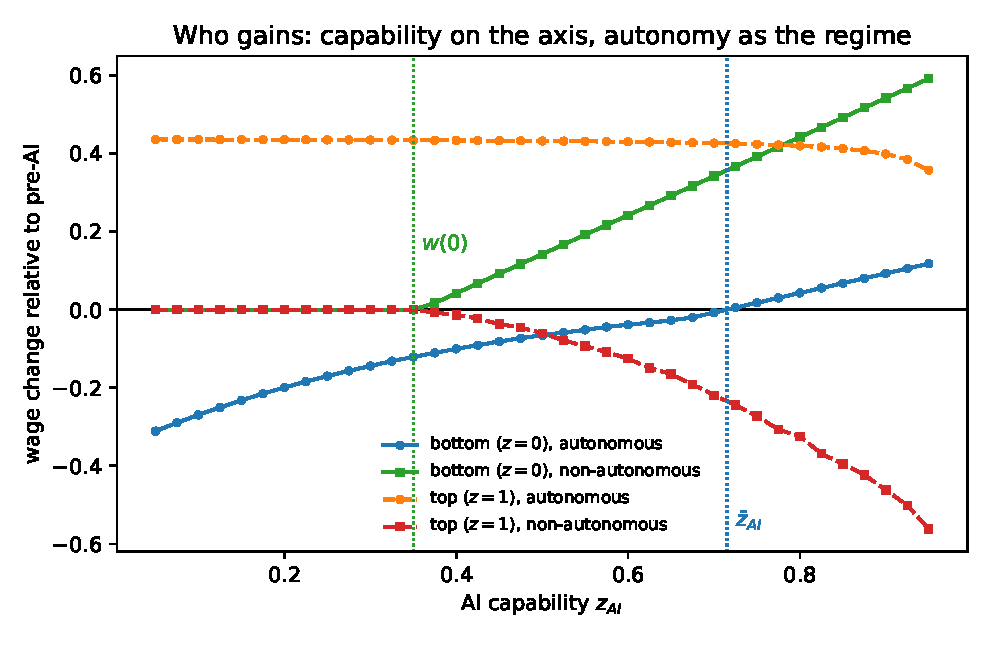
\includegraphics[height=0.8\textheight]{analysis/figures/two_dimensions.pdf}
  \end{center}
\end{frame}

\begin{frame}{3 \textperiodcentered{} Advanced autonomous AI ($z_{AI}=0.85$): winners at both ends (paper's Figure 5b)}
  \begin{center}
    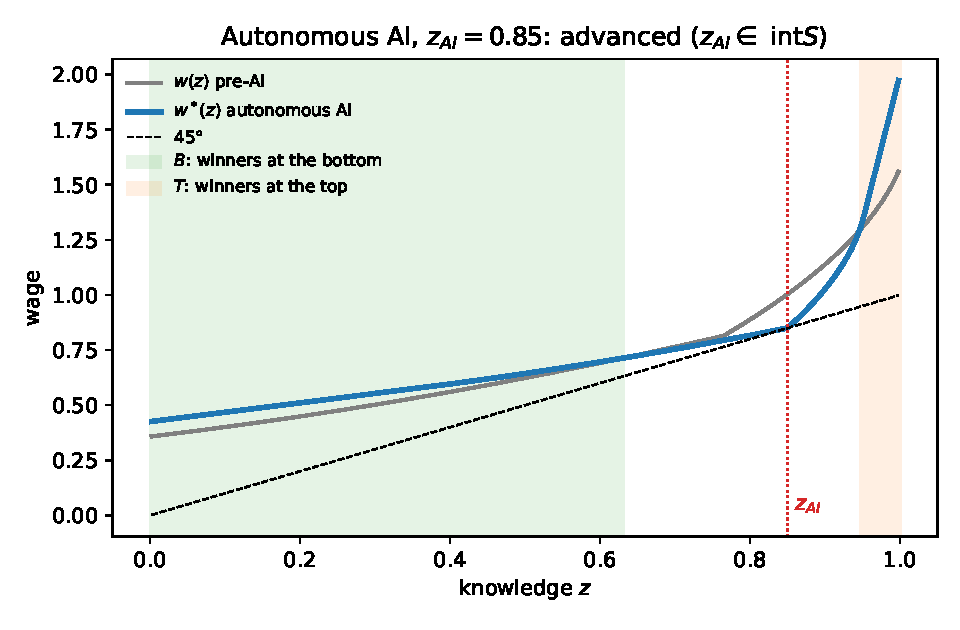
\includegraphics[height=0.8\textheight]{analysis/figures/autonomous_zAI085.pdf}
  \end{center}
\end{frame}

\begin{frame}{3 \textperiodcentered{} Autonomous vs non-autonomous, $z_{AI}=0.85$: Proposition 6 (paper's Figure 9)}
  \begin{center}
    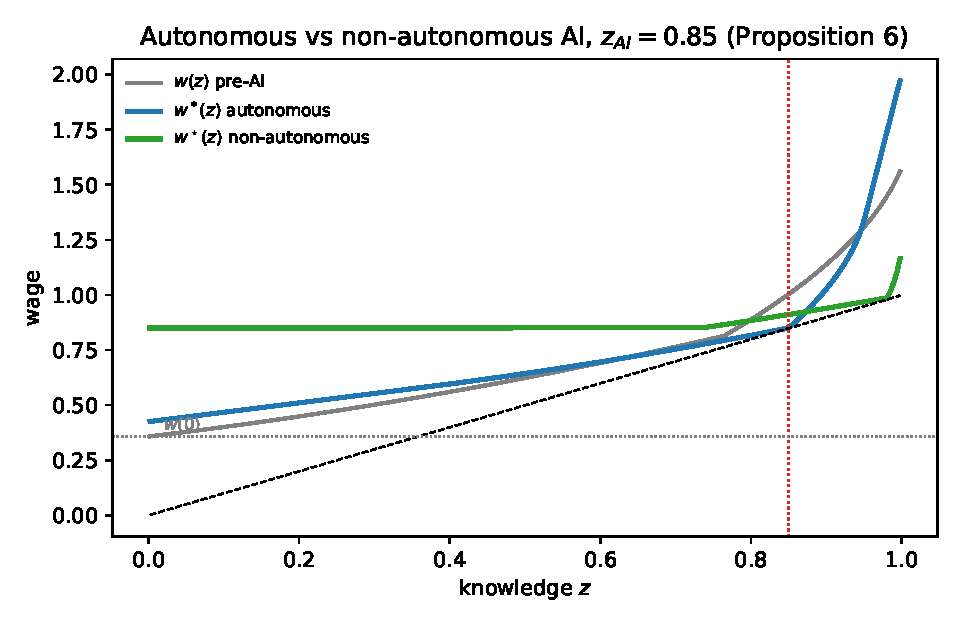
\includegraphics[height=0.8\textheight]{analysis/figures/nonautonomous_zAI085.pdf}
  \end{center}
\end{frame}

%================= 4. LEAN ===========================================
\begin{frame}{4 \textperiodcentered{} Lean I: the run, the statement spec, the status}
  \footnotesize
  \textbf{Workflow (AppliedModelingLib, clone at commit \texttt{2db7d108}).} Pin v11 by SHA-256 $\to$ \texttt{init-spec}
  $\to$ statement spec with 10 targets (page-level locators, literal source statements, exact Lean types) $\to$
  \texttt{paper\_contribution.py new --statement-spec} (the scaffold Lean-validates every Spec) $\to$ proofs in
  \texttt{ProofInterface.lean}, helpers and extension in \texttt{MainTheorems.lean} $\to$
  \texttt{lake build IT25KnowledgeEconomy} $\to$ \texttt{check IT25KnowledgeEconomy --fast}.
  \textbf{Agent:} Claude Code, not Codex (author's decision; disclosed in \texttt{lean/docs/RUN\_LOG.md}).

  \smallskip
  \textbf{The ten Specs} (\texttt{lean/PaperInterface.lean}), all proved, no \texttt{sorry}:
  span of control $n(z)$ as the unique solution of $h\,n(1-z)=1$ (p.\ 10); $n>1$ and strictly increasing on $[0,1)$
  (p.\ 22); the three profit identities (p.\ 12); Prop.\ 2 prices: $r^*=z_{AI}$, $w^*=z_{AI}(1-1/n(z))<z_{AI}$,
  $w^*=n(z_{AI})(s-z_{AI})$ (p.\ 19); ``$z_{AI}$ always loses'' (p.\ 24); non-autonomous $w^\star=z_{AI}$ from
  $r^\star=0$ (p.\ 26); Prop.\ 6.3 comparison $w^\star-w^*=h(1-z)z_{AI}>0$ and $w^\star>w \iff z_{AI}>w$ (p.\ 27);
  Prop.\ 6.1 in idle-compute form (p.\ 27).

  \smallskip
  \textbf{Status: partially formalized.} Existence/uniqueness of equilibrium, the occupational partition (who is in
  $W^*_a$, $S^*_a$, $W^\star_a$), the strict ``$>z$'' in Prop.\ 2 and the threshold $\bar z_{AI}$ of Prop.\ 5 are
  \emph{declared boundaries}; the numerics cover them. \textbf{Result:} \texttt{lake build IT25KnowledgeEconomy}:
  Build completed successfully (3302 jobs); \texttt{check --fast}: exit 0 (\texttt{lean/docs/CHECK\_FAST\_OUTPUT.txt}).
  \textbf{Blocker, stated exactly:} the renamed library's root would not rebuild on my laptop in time (12 h, disk-bound),
  so the paper modules import three Mathlib modules instead of \texttt{import Mathlib}, and the spec validation ran under
  those imports instead of \texttt{import AppliedModelingLib}; no library declaration is used (\texttt{RUN\_LOG.md}).
\end{frame}

\begin{frame}[fragile]{4 \textperiodcentered{} Lean II (required slide): Proposition 2's wage of an AI-assisted worker}
  \scriptsize
  \textbf{Paper (p.\ 12, 19).} Zero profit of a top-automated firm with $r^*=z_{AI}$:
  $\;n(z)\,[z_{AI}-w^*(z)]-z_{AI}=0\ \Rightarrow\ w^*(z)=z_{AI}\big(1-\tfrac1{n(z)}\big),\ n(z)=\tfrac{1}{h(1-z)}$.
  \vspace{-2pt}
  \begin{lstlisting}[basicstyle=\ttfamily\tiny]
def paper_prop2_ai_assisted_worker_wageSpec : Prop :=
  ∀ h z zAI w : ℝ, 0 < h → h < 1 → 0 ≤ z → z < 1 → 0 < zAI →
    (1 / (h * (1 - z))) * (zAI - w) - zAI = 0 →
      w = zAI * (1 - 1 / (1 / (h * (1 - z)))) ∧ w < zAI

theorem paper_prop2_ai_assisted_worker_wage : paper_prop2_ai_assisted_worker_wageSpec := by
  intro h z zAI w hh hh1 hz0 hz1 hzAI hzero
  have hpos : 0 < h * (1 - z) := mul_pos hh (by linarith)
  have hn : 1 / (1 / (h * (1 - z))) = h * (1 - z) := by rw [one_div_one_div]
  have hw : w = zAI - h * (1 - z) * zAI := by
    have hh' : h ≠ 0 := hh.ne'
    have h1z : (1 - z) ≠ 0 := (sub_pos.mpr hz1).ne'
    field_simp at hzero        -- clears the denominator: zAI - w = h (1 - z) zAI
    linarith [hzero]
  refine ⟨?_, ?_⟩
  · rw [hn, hw]; ring
  · rw [hw]; have : 0 < h * (1 - z) * zAI := mul_pos hpos hzAI; linarith
  \end{lstlisting}
  \vspace{-4pt}
  \textbf{Reading.} $h,z,z_{AI},w$ are reals; $n(z)$ is spelled out as \texttt{1 / (h * (1 - z))}; the hypothesis is
  the zero-profit display itself. \texttt{field\_simp at hzero} is the nontrivial step: it multiplies the display by
  $h(1-z)$ --- it needs $h\neq0$ and $1-z\neq0$ as \emph{separate} facts --- then \texttt{linarith} isolates $w$.
  Lean verifies the formula \emph{exactly} from zero profit and
  $r^*=z_{AI}$, and adds $w^*<z_{AI}$. Not verified: the paper's ``$>z$'' on $W^*_a$ --- it needs which humans choose
  the AI-assisted firm, i.e.\ the equilibrium. \texttt{lake build}: success; \texttt{check --fast}: exit 0.
\end{frame}

\begin{frame}[fragile]{4 \textperiodcentered{} Lean III: the two-type extension --- capability thresholds in both regimes}
  \scriptsize
  \textbf{Claim (README).} Two types $z_L<z_{AI}<z_H$, L abundant. Autonomous: the bottom gains iff
  $z_{AI}(1-h(1-z_L))>z_L \iff z_{AI}>\dfrac{z_L}{1-h(1-z_L)}$, a threshold strictly above $z_L$.
  Non-autonomous: gains iff $z_{AI}>z_L$; the non-autonomous premium is the AI solver's share $h(1-z_L)z_{AI}$.
  \vspace{-2pt}
  \begin{lstlisting}[basicstyle=\ttfamily\tiny]
theorem two_type_bottom_gains_autonomous_iff (h zL zAI : ℝ)
    (hh : 0 < h) (hh1 : h < 1) (hL0 : 0 ≤ zL) (hL1 : zL < 1) :
    zL < zAI - h * (1 - zL) * zAI ↔ zL / (1 - h * (1 - zL)) < zAI := by
  have hden : 0 < 1 - h * (1 - zL) := by nlinarith
  rw [div_lt_iff₀ hden]
  constructor <;> intro hx <;> nlinarith

theorem two_type_threshold_above_zL (h zL : ℝ) (hh : 0 < h) (hh1 : h < 1)
    (hL0 : 0 < zL) (hL1 : zL < 1) : zL < zL / (1 - h * (1 - zL)) := by
  have hden : 0 < 1 - h * (1 - zL) := by nlinarith
  rw [lt_div_iff₀ hden]; nlinarith

theorem two_type_nonautonomous_bottom_premium (h zL zAI : ℝ) (hh : 0 < h) (hL1 : zL < 1)
    (hzAI : 0 < zAI) : zAI - h * (1 - zL) * zAI < zAI := by
  have : 0 < h * (1 - zL) * zAI := mul_pos (mul_pos hh (by linarith)) hzAI; linarith
  \end{lstlisting}
  \textbf{Reading.} \texttt{div\_lt\_iff₀} turns the threshold inequality into a product inequality once the
  denominator $1-h(1-z_L)>0$ is established (\texttt{nlinarith} from $h<1$, $z_L<1$). The LP gives the same
  threshold numerically ($0.4615$ for $z_L=0.3$, $h=1/2$). This is my extension, not a printed statement of the paper.
\end{frame}

%================= 5. DONDE NO LE CREI A LA IA =======================
\begin{frame}{5 \textperiodcentered{} Where I did not believe the AI}
  \begin{columns}[T]
    \column{0.30\textwidth}
      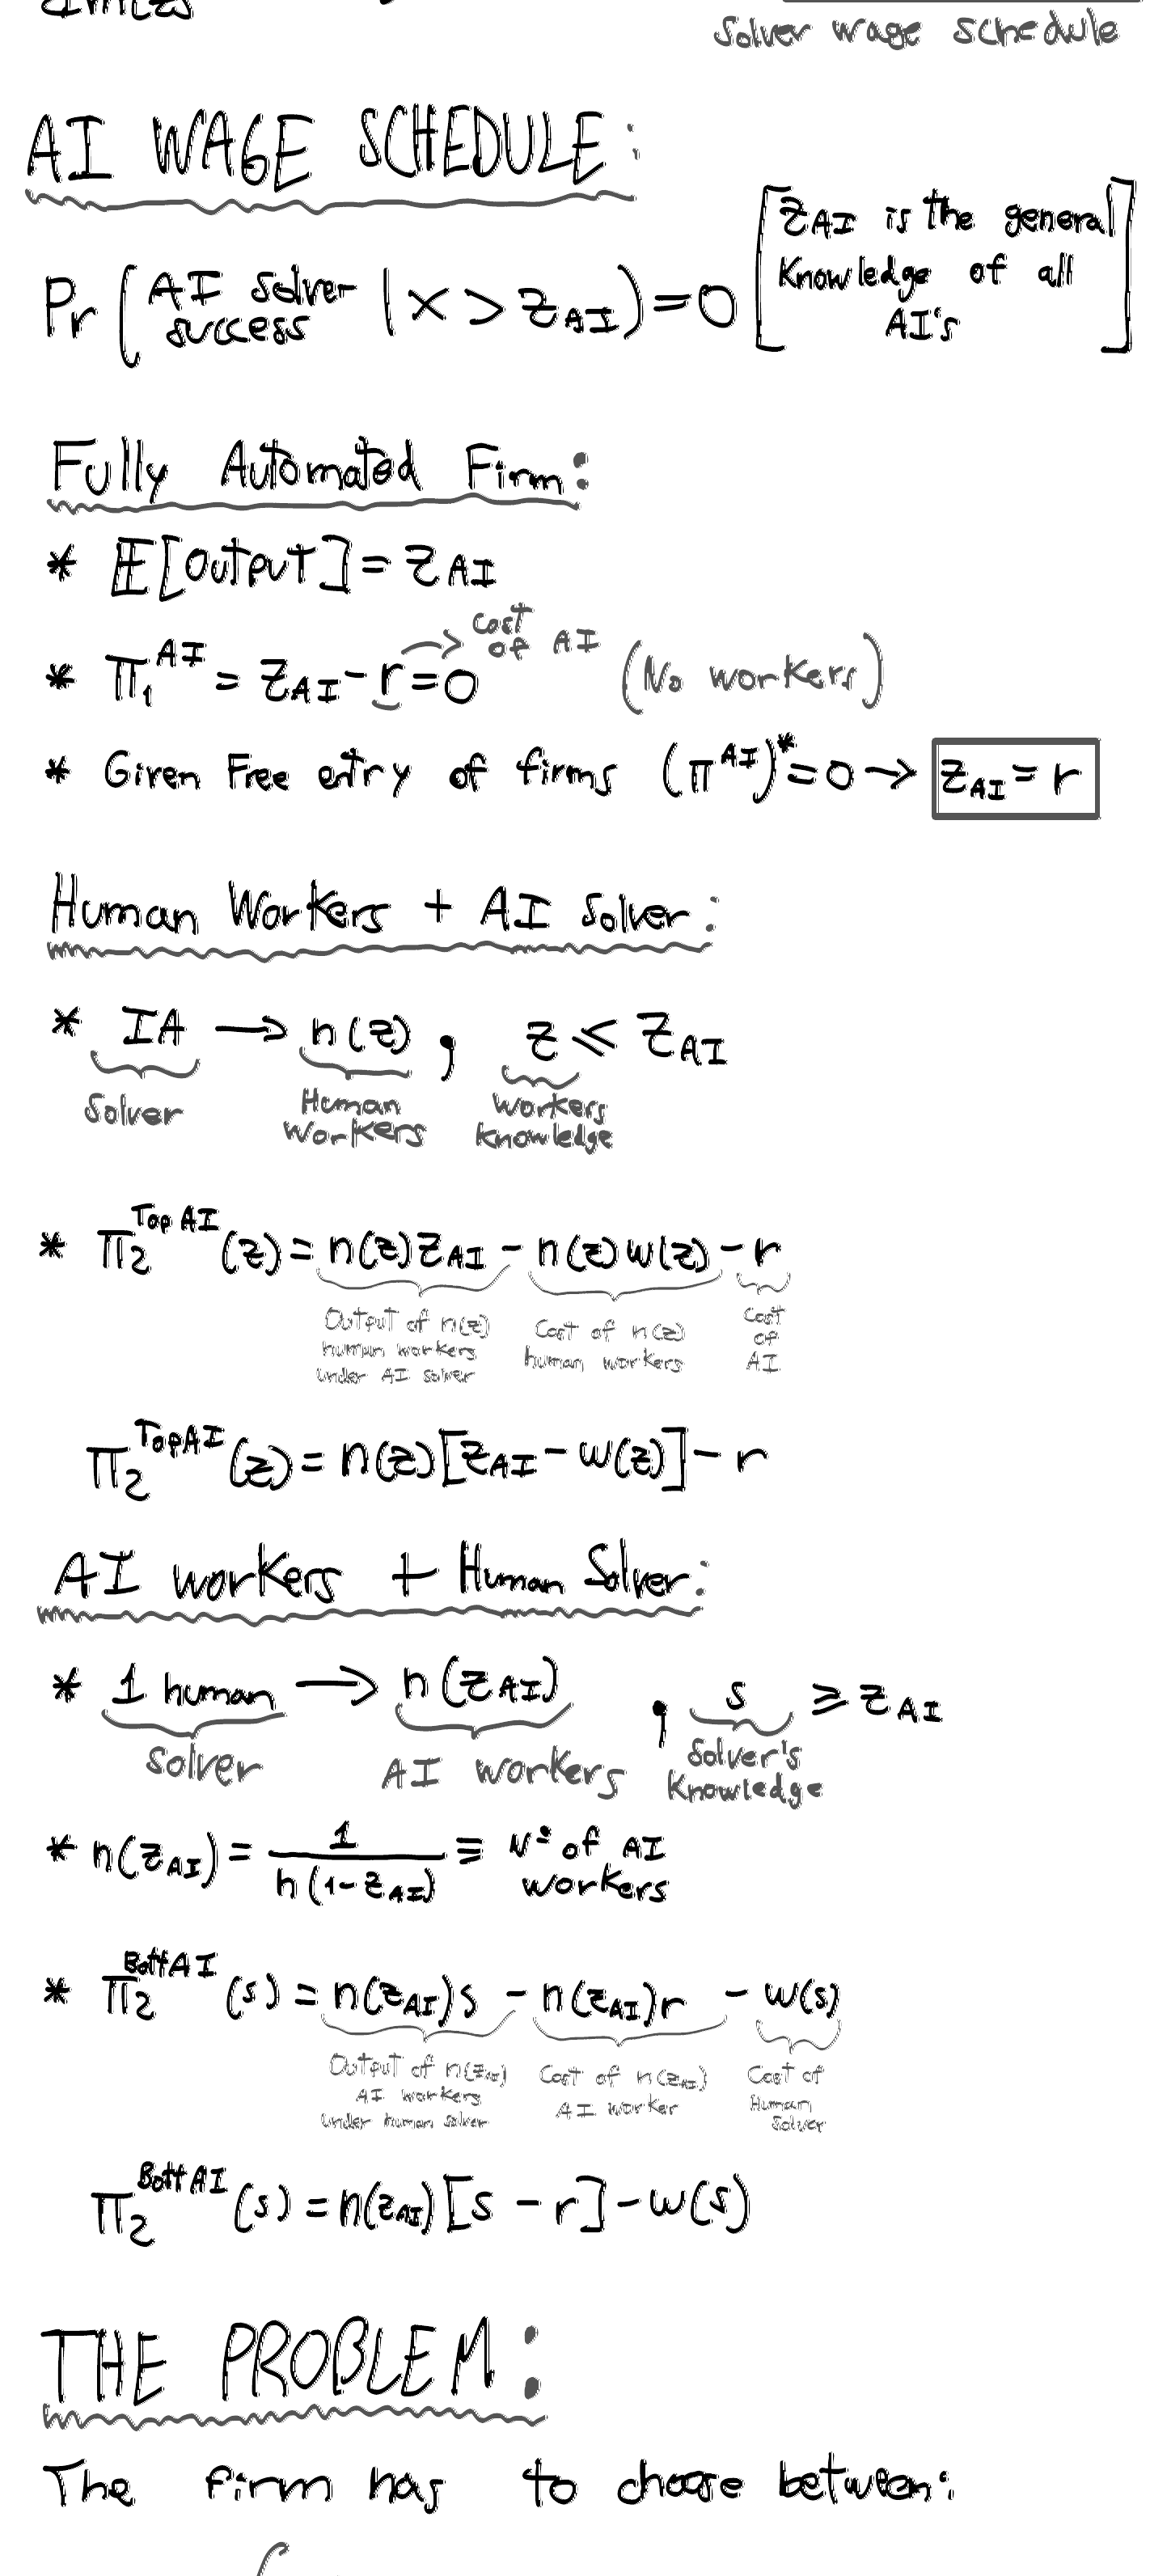
\includegraphics[height=0.66\textheight]{hand/hand-ide-talamas-2025-part3.png}
      \\[2pt]{\scriptsize Part 3 of the hand derivation: $r=z_{AI}$ and the two AI wage formulas. Full page in the backup.}
    \column{0.68\textwidth}\footnotesize
      \textbf{Claim 1 (ChatGPT, closing summary of the study session, \texttt{prompts.md} Session 1):}
      ``AI capability determina la dirección de la reasignación ocupacional; \emph{AI autonomy determina quién
      captura principalmente las ganancias}.'' --- the one-dimensional gloss. Against Proposition 5: with autonomous AI
      the bottom captures gains \emph{only if} $z_{AI}>\bar z_{AI}$; against Proposition 6: without autonomy, only if
      $z_{AI}>w(0)$. \textbf{Verdict: incomplete} --- autonomy sets who gains \emph{more}; capability sets whether the
      bottom gains at all.

      \smallskip
      \textbf{Claim 2 (ChatGPT):} $w^*(z)=z_{AI}(1-1/n(z))$ and $w^*(s)=n(z_{AI})(s-z_{AI})$ ``from zero profit''.
      Checked by hand (photo) and in Lean: \textbf{correct}, and the same algebra gives $w^\star(z)=z_{AI}$ when $r^\star=0$.

      \smallskip
      \textbf{Claim 3 (my own LP).} LP duals = equilibrium wages. Against Proposition 1's closed form ($G(z)=z$,
      $h=1/2$): $w(1)=1.578$ vs LP $1.56$ (grid ends at $0.998$), $w(0)=0.357$ vs $0.358$. \textbf{Verdict: right.}

      \smallskip
      \textbf{Claim 4 (Lean pushed back).} Proposition 2's ``$w^*(z)=z_{AI}(1-1/n(z))>z$'': from zero profit alone the
      ``$>z$'' is \emph{not} provable (it depends on who is in $W^*_a$). Formula proved, inequality declared a boundary.
  \end{columns}
\end{frame}

\begin{frame}{5 \textperiodcentered{} The trap, the versions, and what to carry away}
  \footnotesize
  \begin{itemize}
    \item \textbf{Trap.} ``Driven by autonomy, not capability'' collapses a $2\times2$ taxonomy (basic/advanced $\times$
      autonomous/non-autonomous). The winners-at-the-bottom condition is a capability threshold in both regimes;
      autonomy moves the threshold, the size of the gain, the top's fate and output.
    \item \textbf{Versions.} v11 (Feb 2025, 35 pp.) pinned for Lean; v12 (May 2025, 39 pp.) is the course PDF; JPE
      133(12) 3762--3800 is the published one (ChatGPT session cites its pages). Same Propositions 1--6.
      Talam\textbf{à}s, 2025 --- not the 2024 working paper.
    \item \textbf{Lean.} Ten Specs proved: prices and wages follow \emph{exactly} from zero profit once $r$ is pinned by
      abundant compute; the distributional propositions need the equilibrium partition, which is the declared boundary.
    \item \textbf{Numerics.} The efficient equilibrium is an LP; its duals reproduce the paper's figures and give
      $\bar z_{AI}\approx0.715$, $w(0)=0.358$.
    \item \textbf{One sentence.} A co-pilot democratises knowledge, a co-worker scales the expert's --- but only an AI
      good enough to beat the bottom's outside option helps the bottom at all.
  \end{itemize}
\end{frame}

%================= BACKUP: FIGURAS (una por slide, centradas) =========
\begin{frame}{B1 \textperiodcentered{} Pre-AI equilibrium, $G(z)=z$, $h=1/2$ (paper's Figure 3a)}
  \begin{center}
    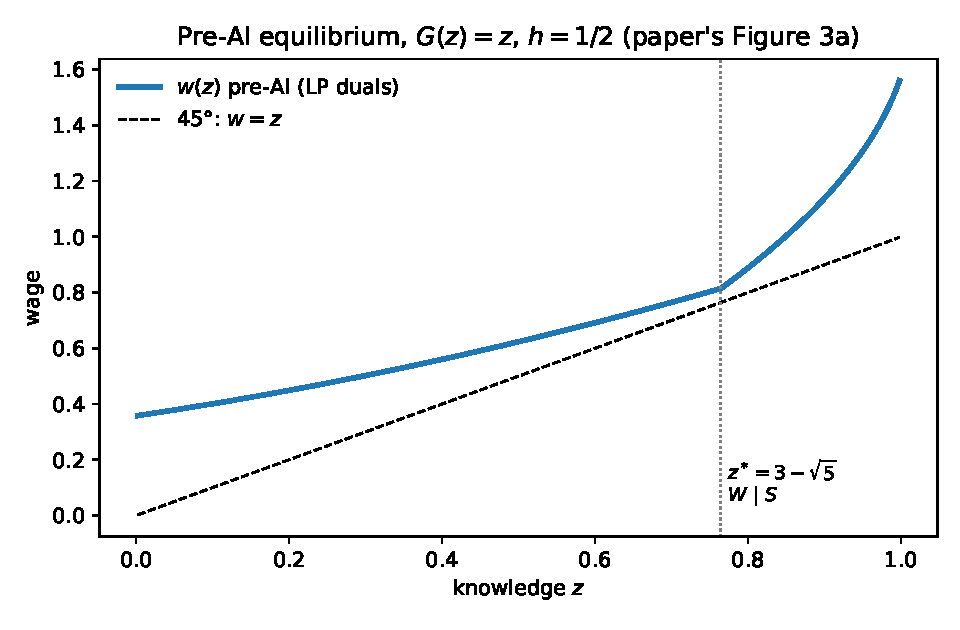
\includegraphics[height=0.8\textheight]{analysis/figures/pre_ai_wages.pdf}
  \end{center}
\end{frame}

\begin{frame}{B2 \textperiodcentered{} Basic autonomous AI ($z_{AI}=0.425$): winners only at the top (Figure 5a)}
  \begin{center}
    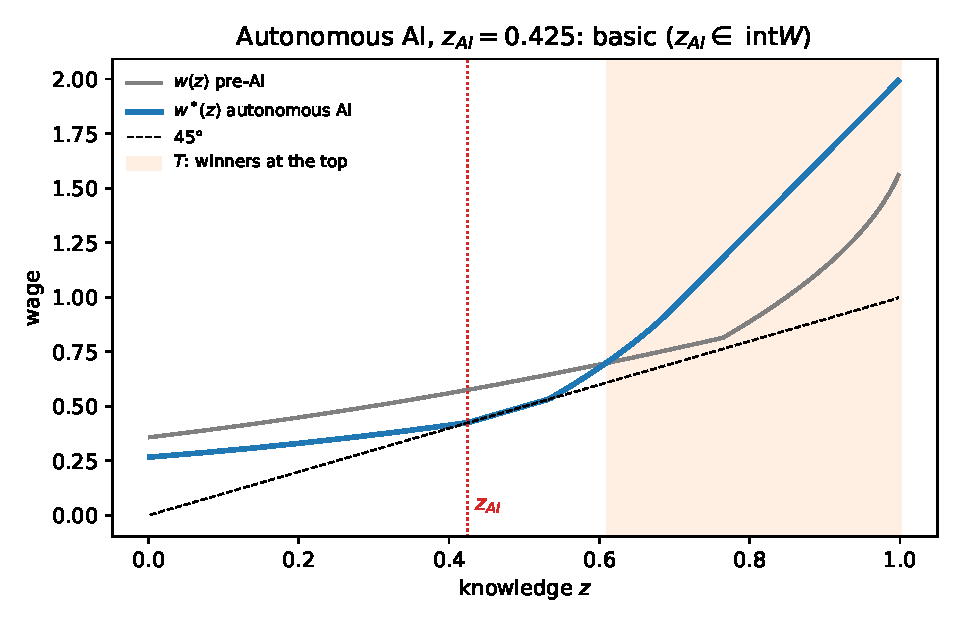
\includegraphics[height=0.8\textheight]{analysis/figures/autonomous_zAI0425.pdf}
  \end{center}
\end{frame}

\begin{frame}{B3 \textperiodcentered{} Autonomous vs non-autonomous, $z_{AI}=0.425$}
  \begin{center}
    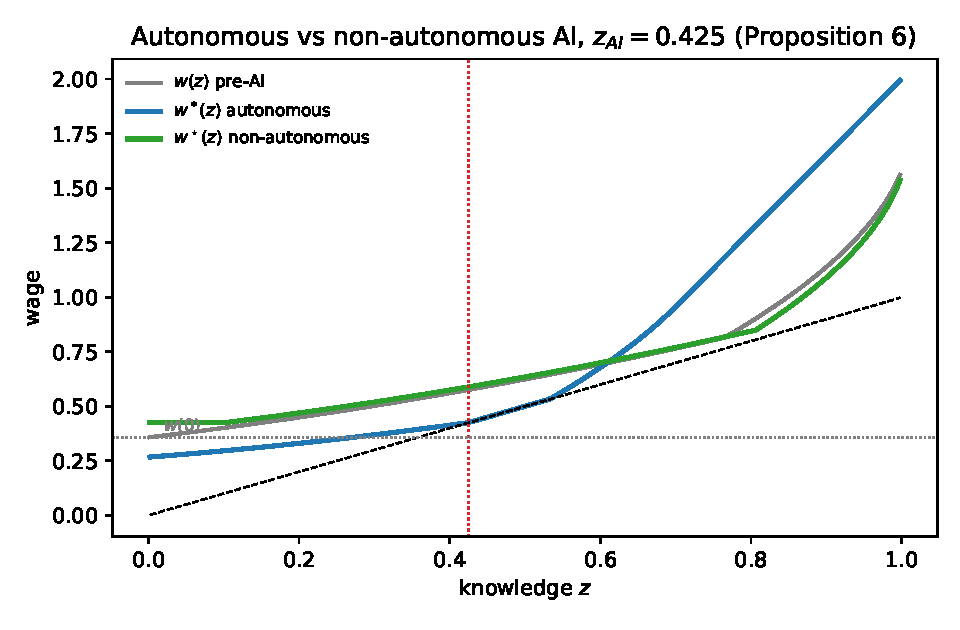
\includegraphics[height=0.8\textheight]{analysis/figures/nonautonomous_zAI0425.pdf}
  \end{center}
\end{frame}

\begin{frame}{B4 \textperiodcentered{} Output: autonomous above non-autonomous for every $z_{AI}$ (Proposition 6.1)}
  \begin{center}
    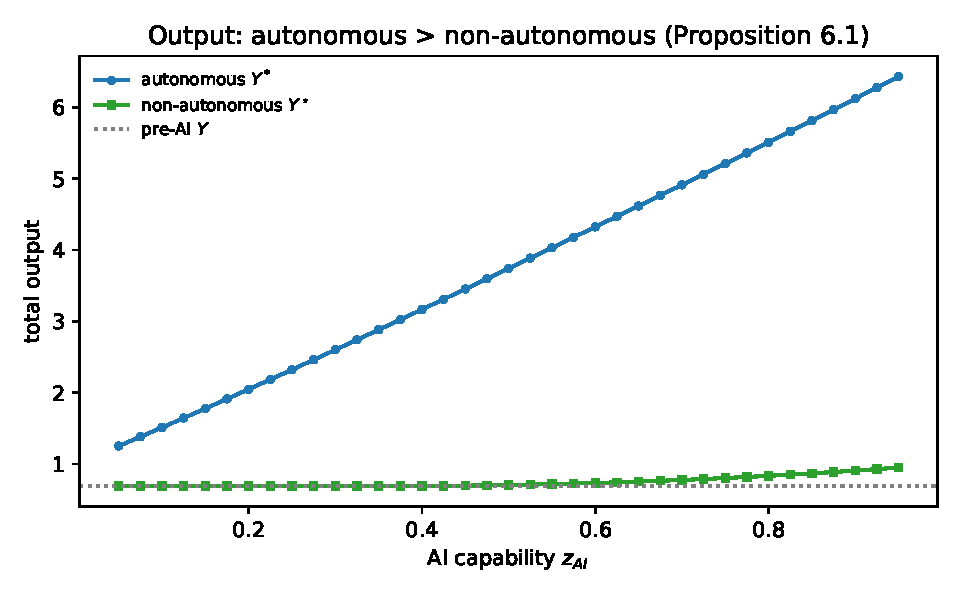
\includegraphics[height=0.8\textheight]{analysis/figures/output_comparison.pdf}
  \end{center}
\end{frame}

\begin{frame}{B5 \textperiodcentered{} Two-type economy: the thresholds $z_L/(1-h(1-z_L))$ and $z_L$}
  \begin{center}
    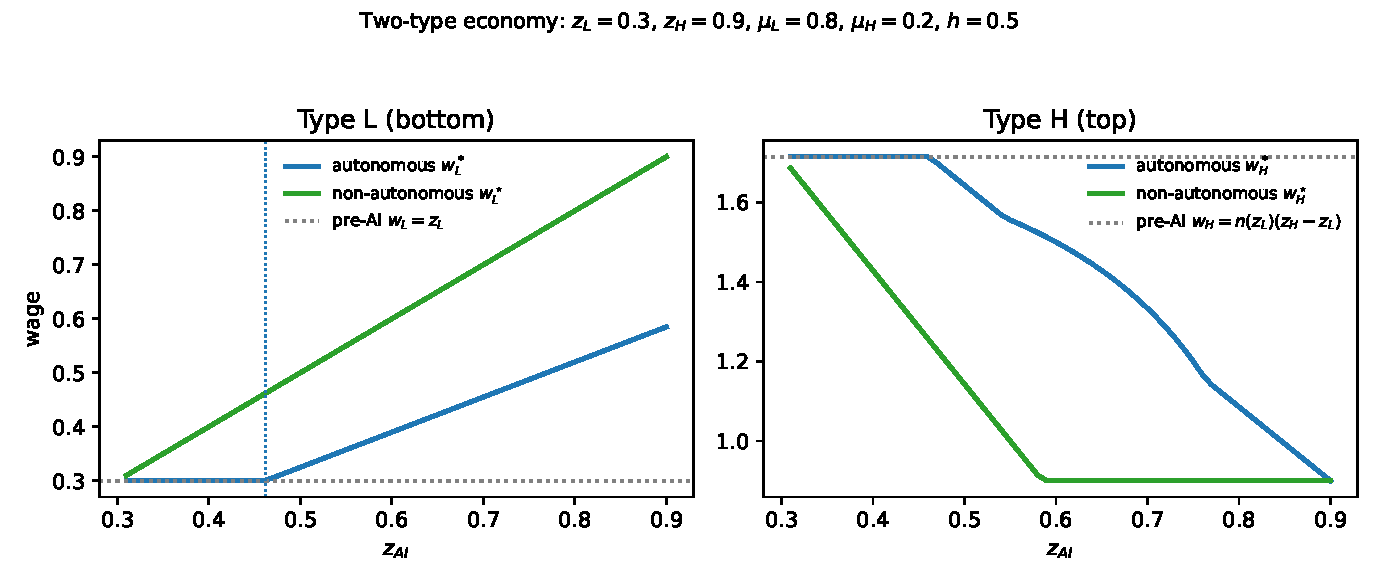
\includegraphics[height=0.8\textheight]{analysis/figures/two_type.pdf}
  \end{center}
\end{frame}

%================= BACKUP: DERIVACION A MANO ==========================
\begin{frame}{B6 \textperiodcentered{} Hand derivation 1/5: assumptions and the pre-AI firm problem}
  \begin{center}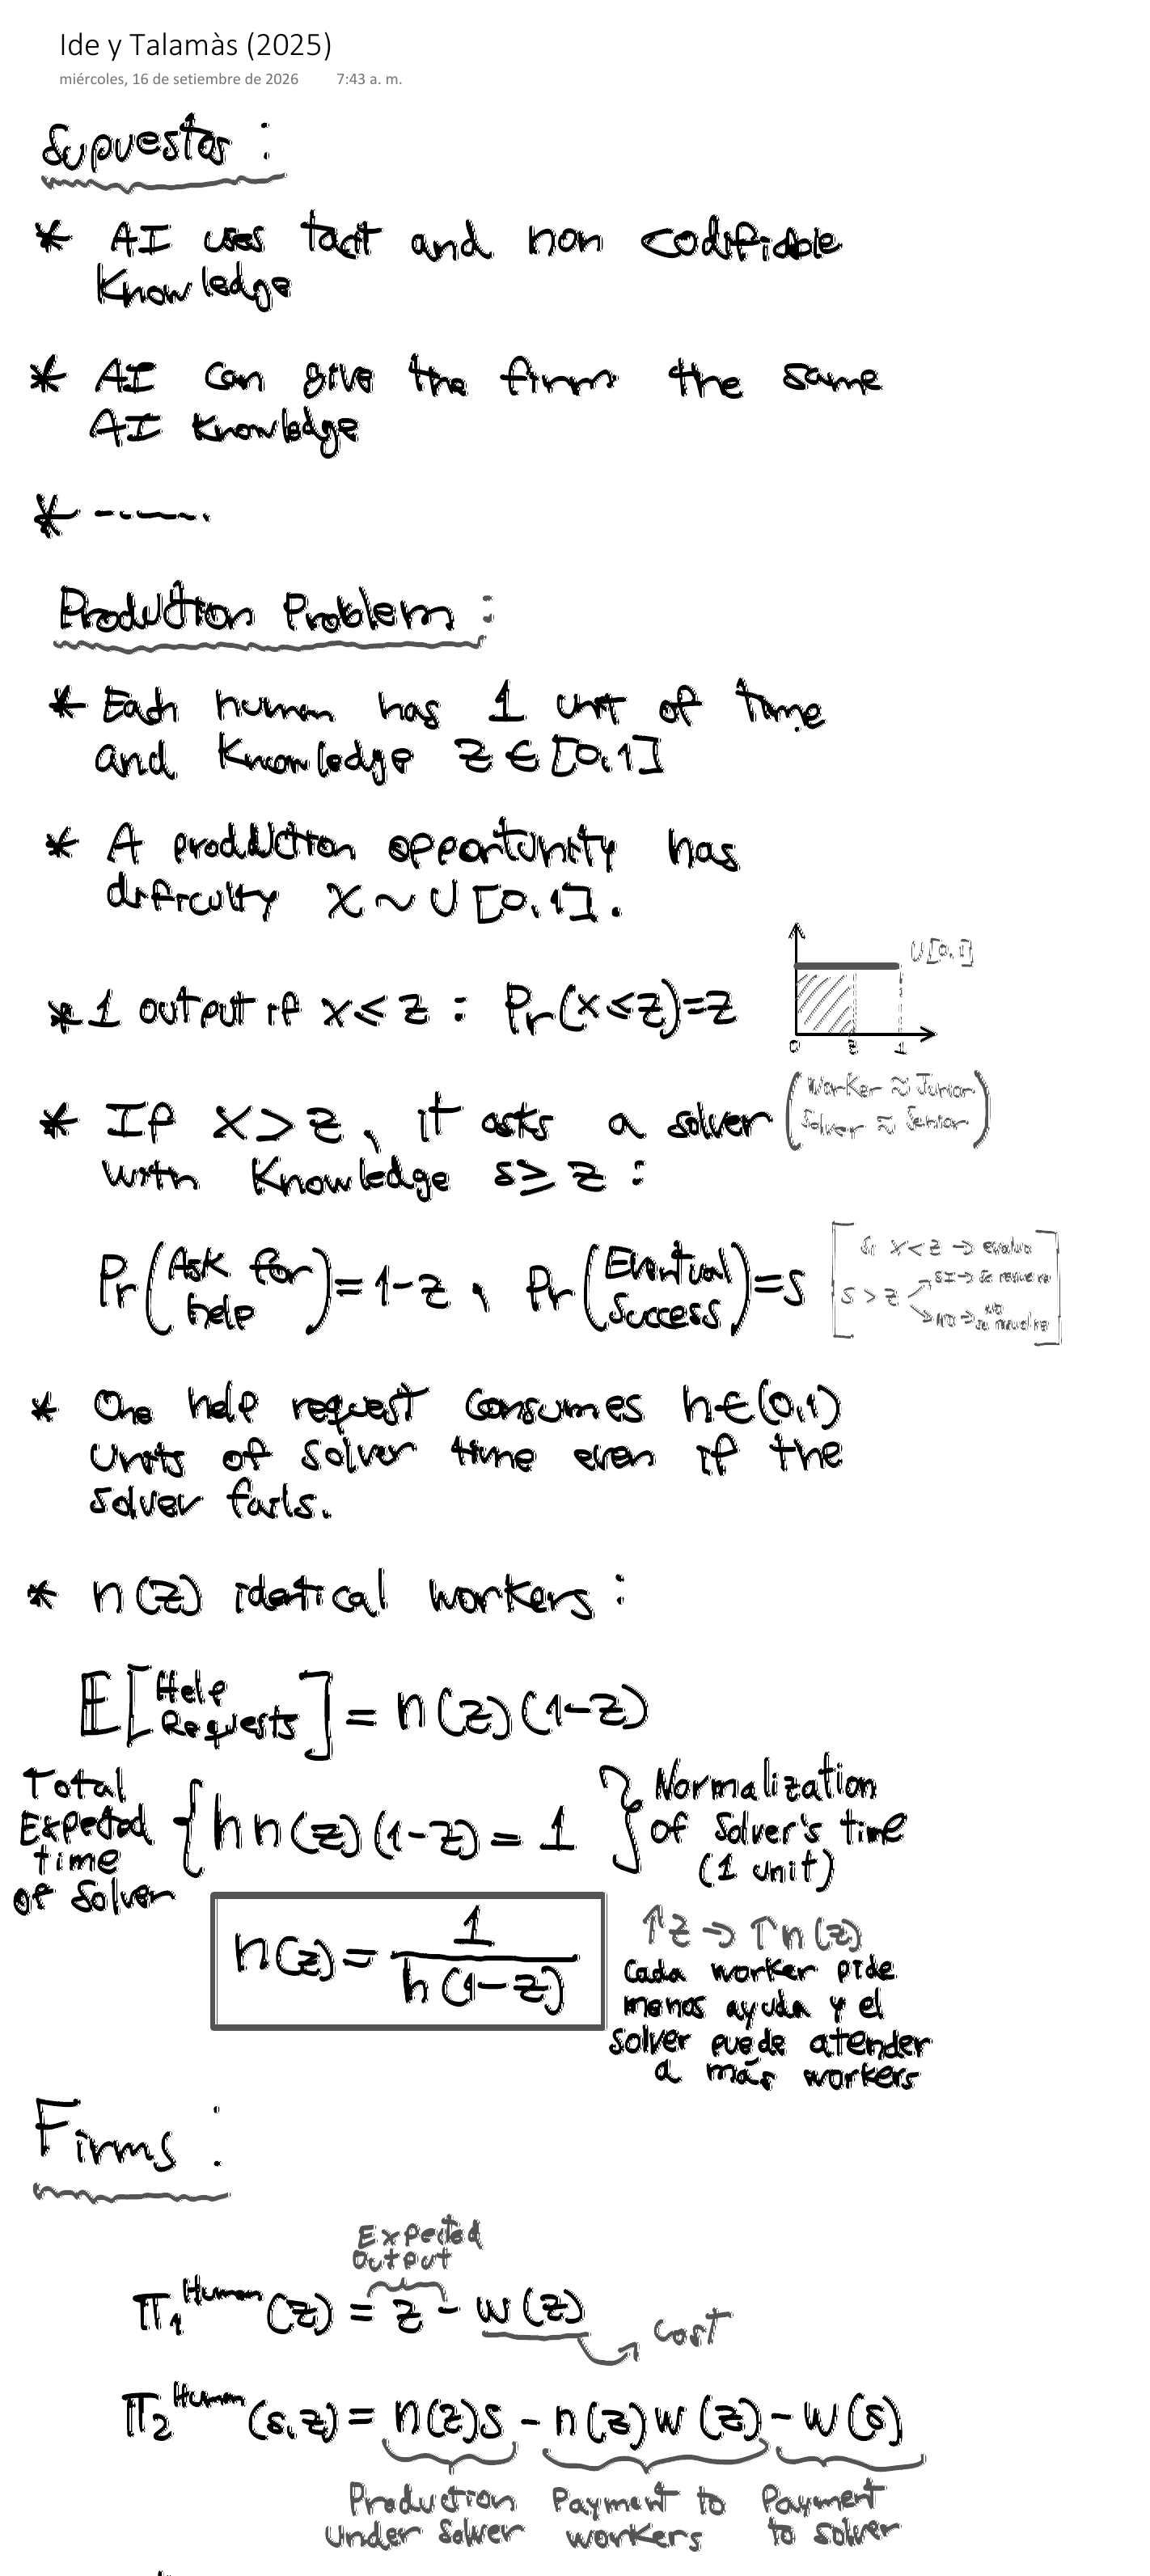
\includegraphics[height=0.84\textheight]{hand/hand-ide-talamas-2025-part1.png}\end{center}
\end{frame}
\begin{frame}{B7 \textperiodcentered{} Hand derivation 2/5: profits, competitive equilibrium, pre-AI wage schedule}
  \begin{center}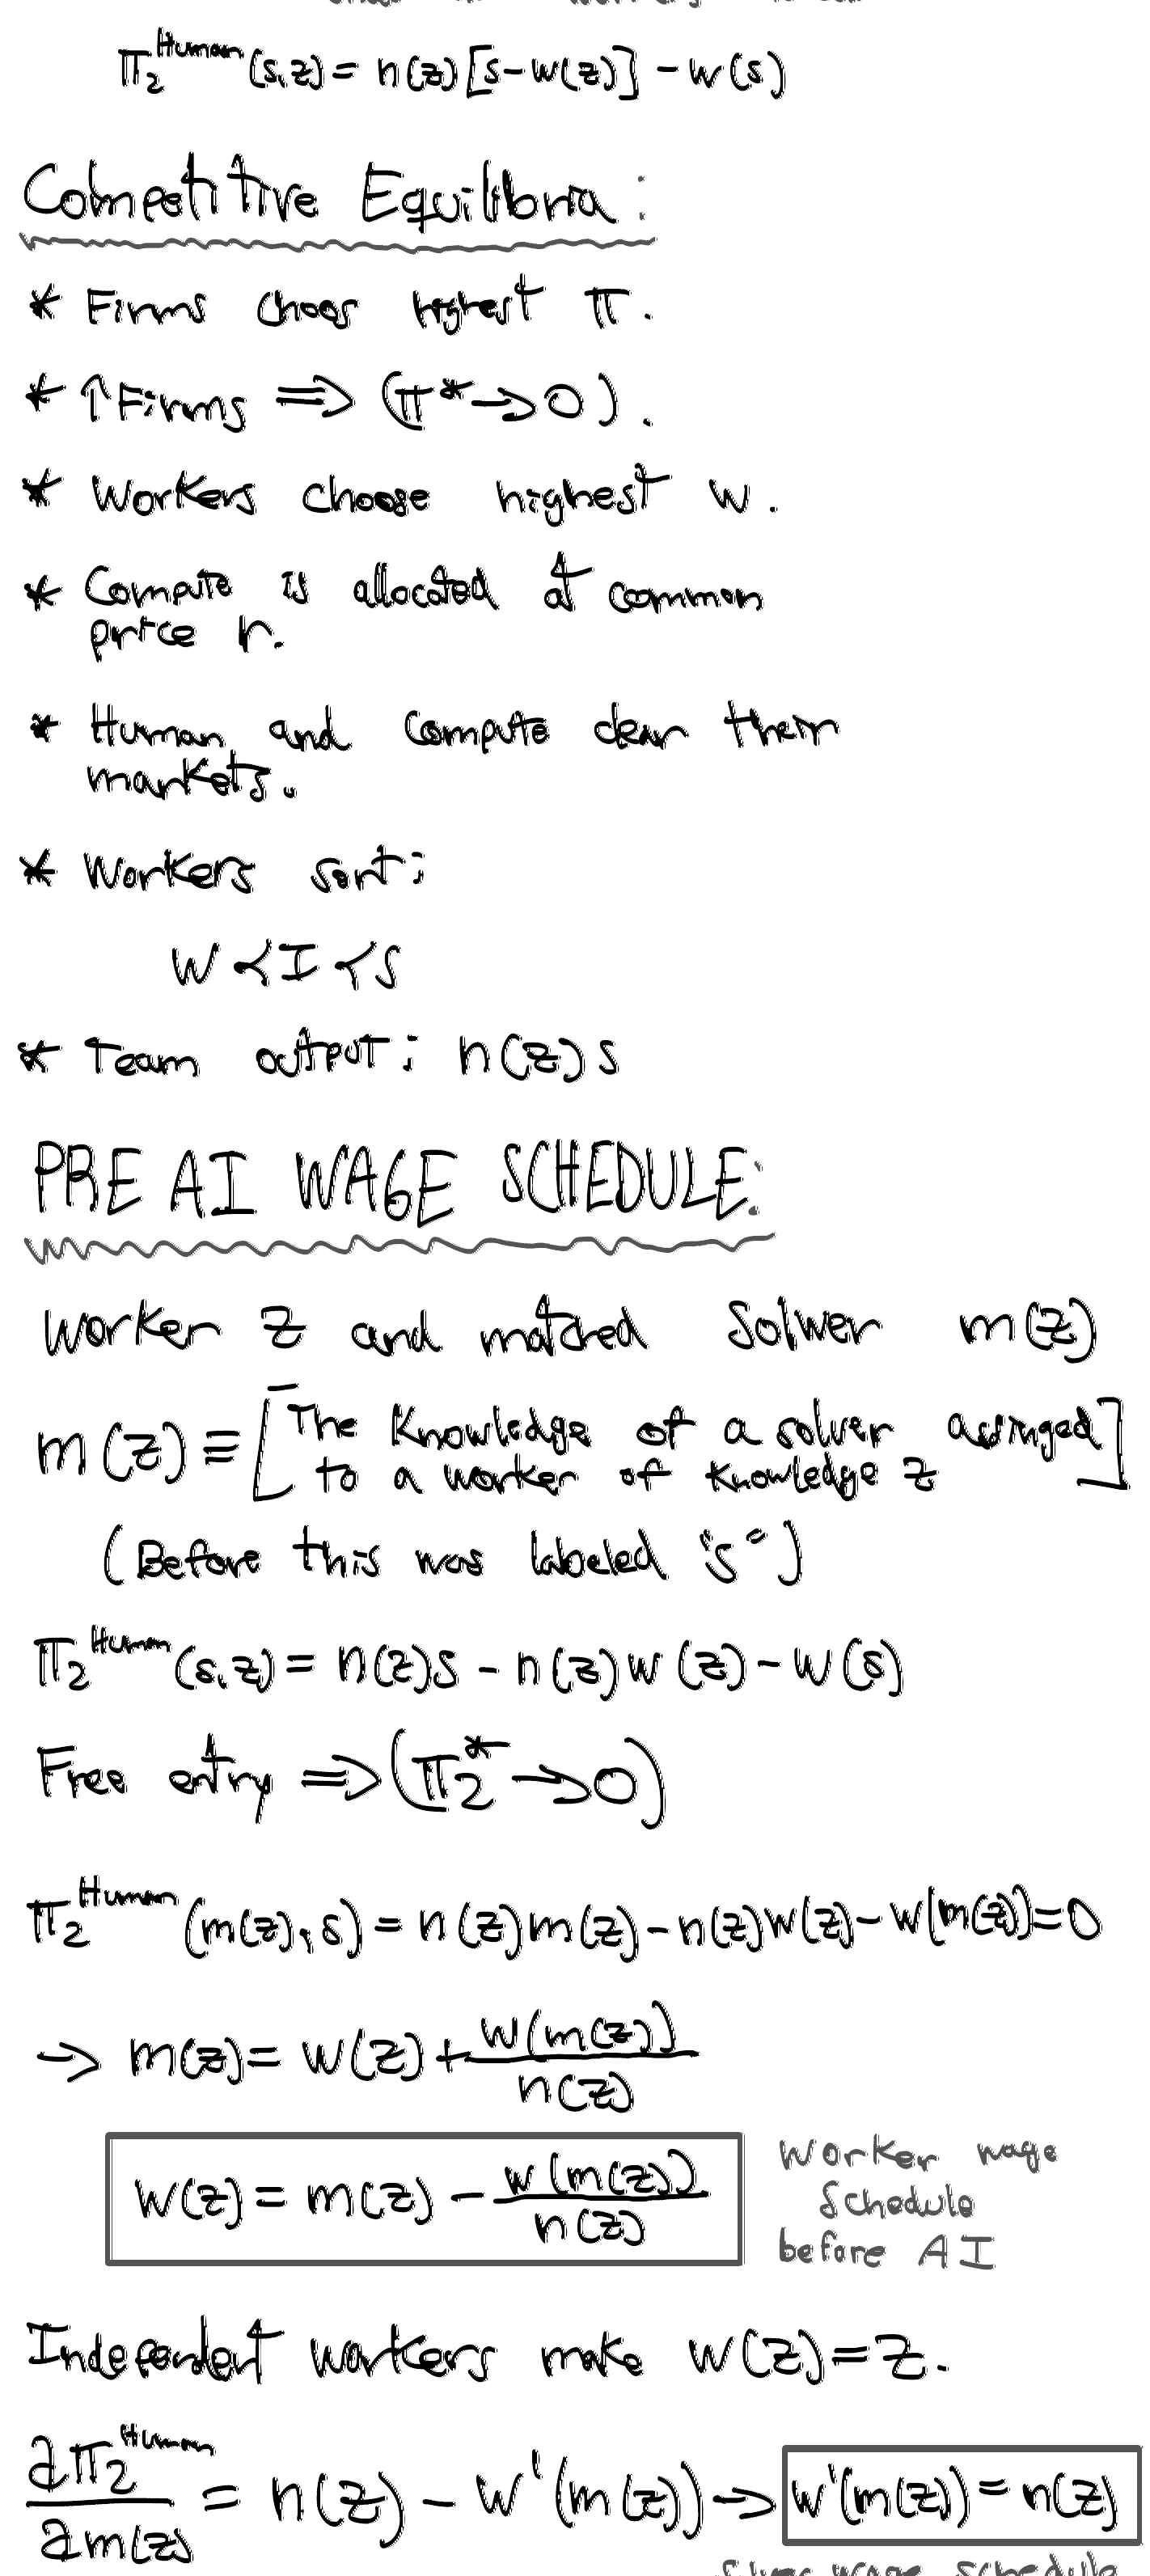
\includegraphics[height=0.84\textheight]{hand/hand-ide-talamas-2025-part2.png}\end{center}
\end{frame}
\begin{frame}{B8 \textperiodcentered{} Hand derivation 3/5: $r=z_{AI}$ and the AI wage schedule}
  \begin{center}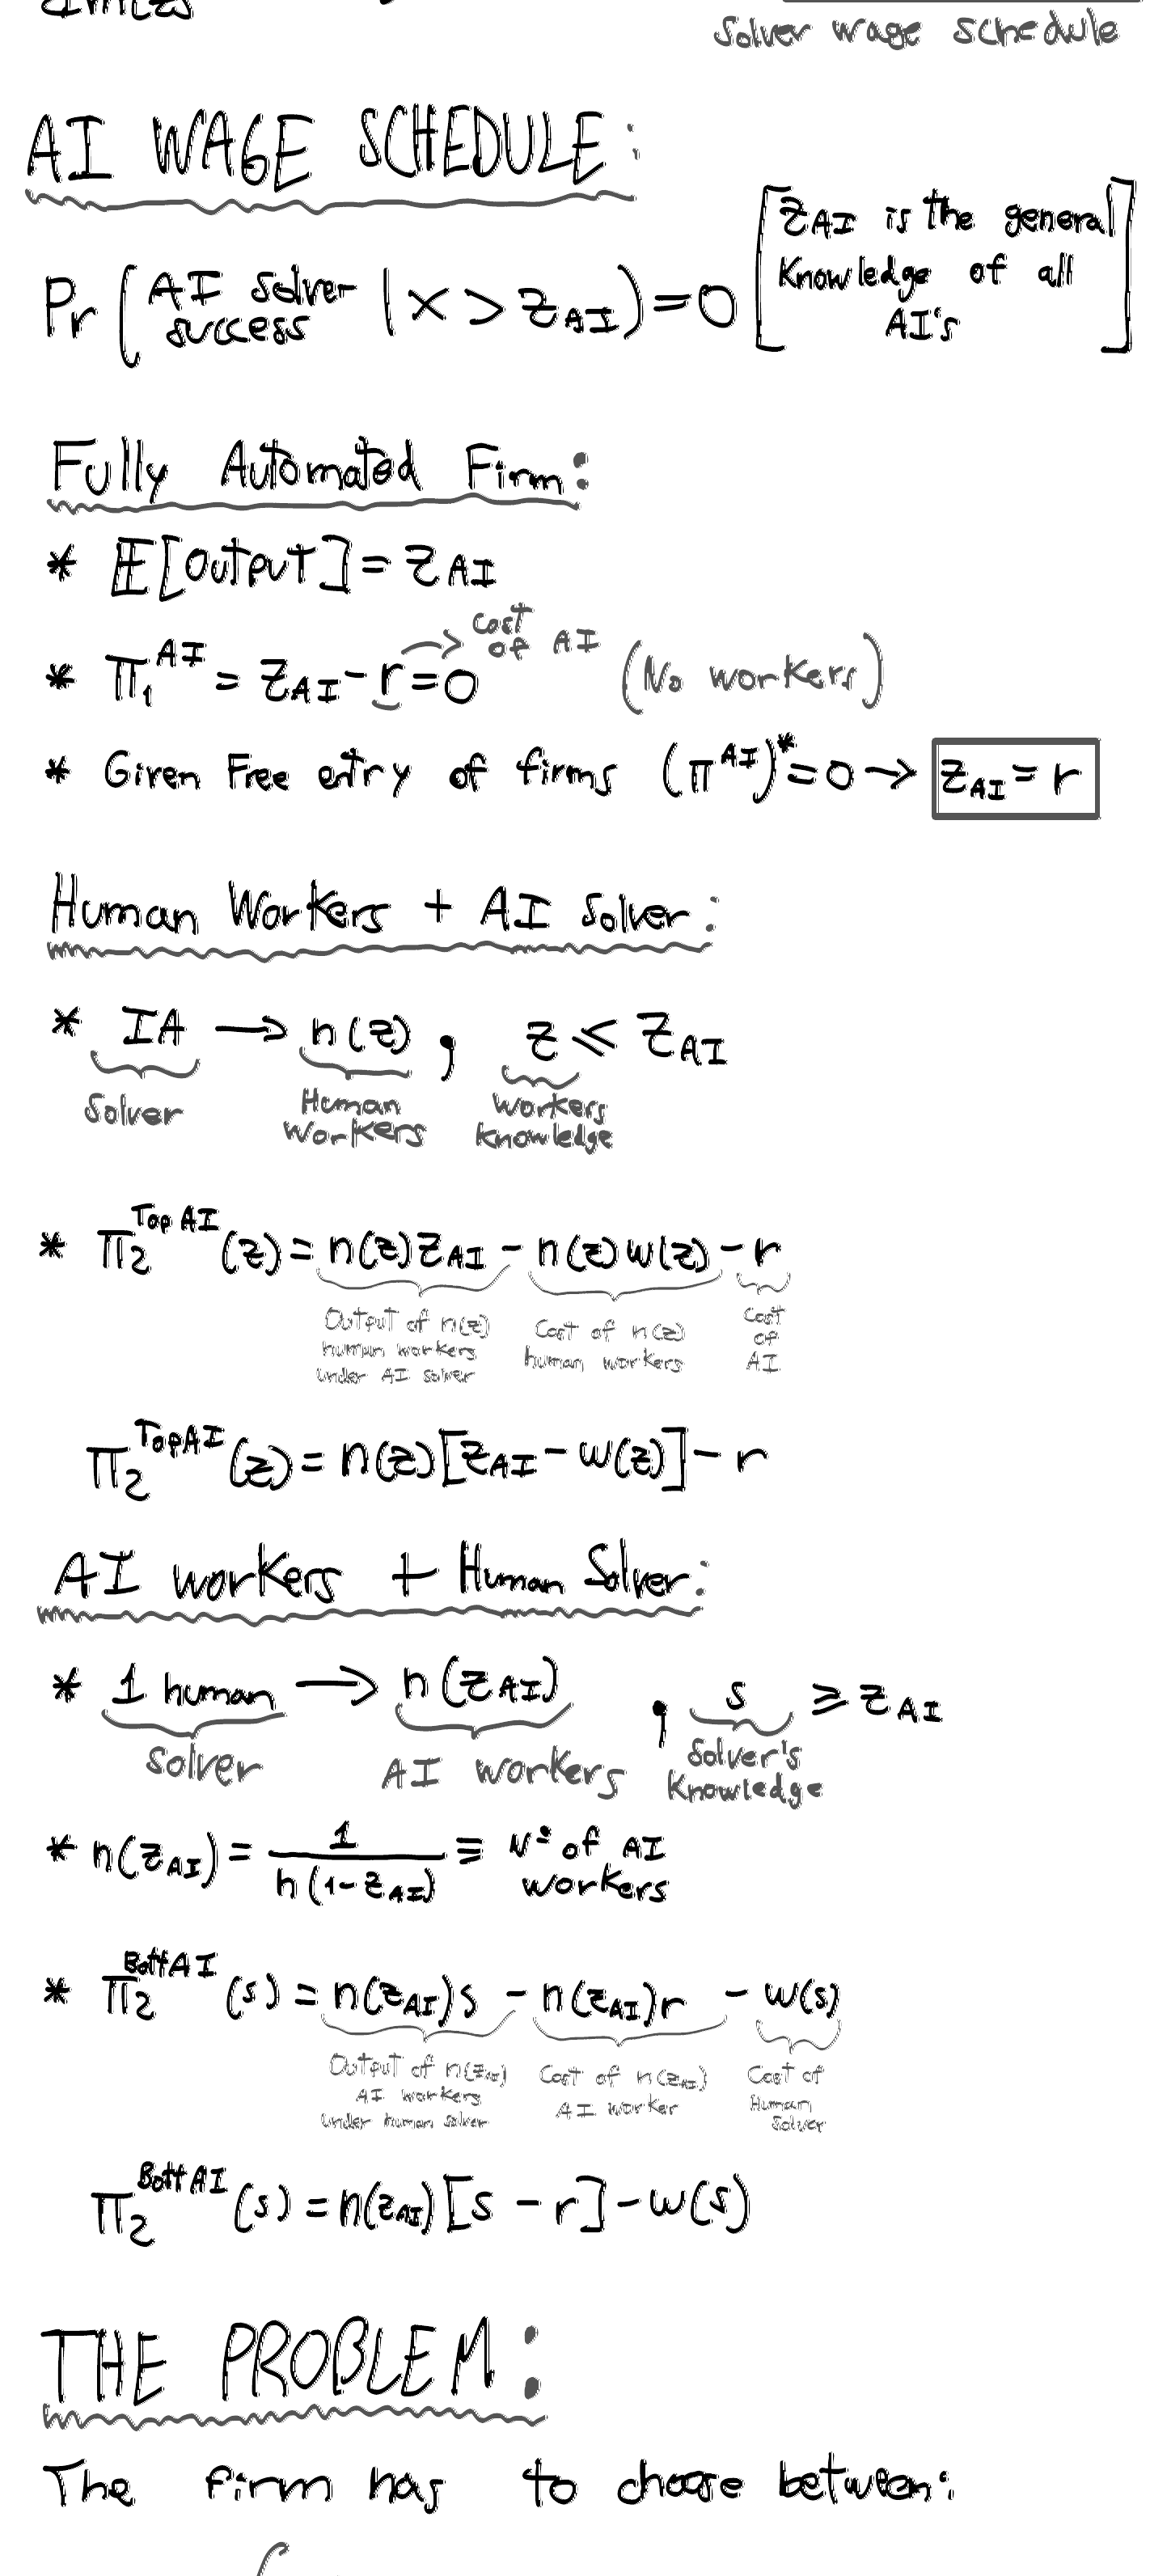
\includegraphics[height=0.84\textheight]{hand/hand-ide-talamas-2025-part3.png}\end{center}
\end{frame}
\begin{frame}{B9 \textperiodcentered{} Hand derivation 4/5: the firm's problem and the compute accounting}
  \begin{center}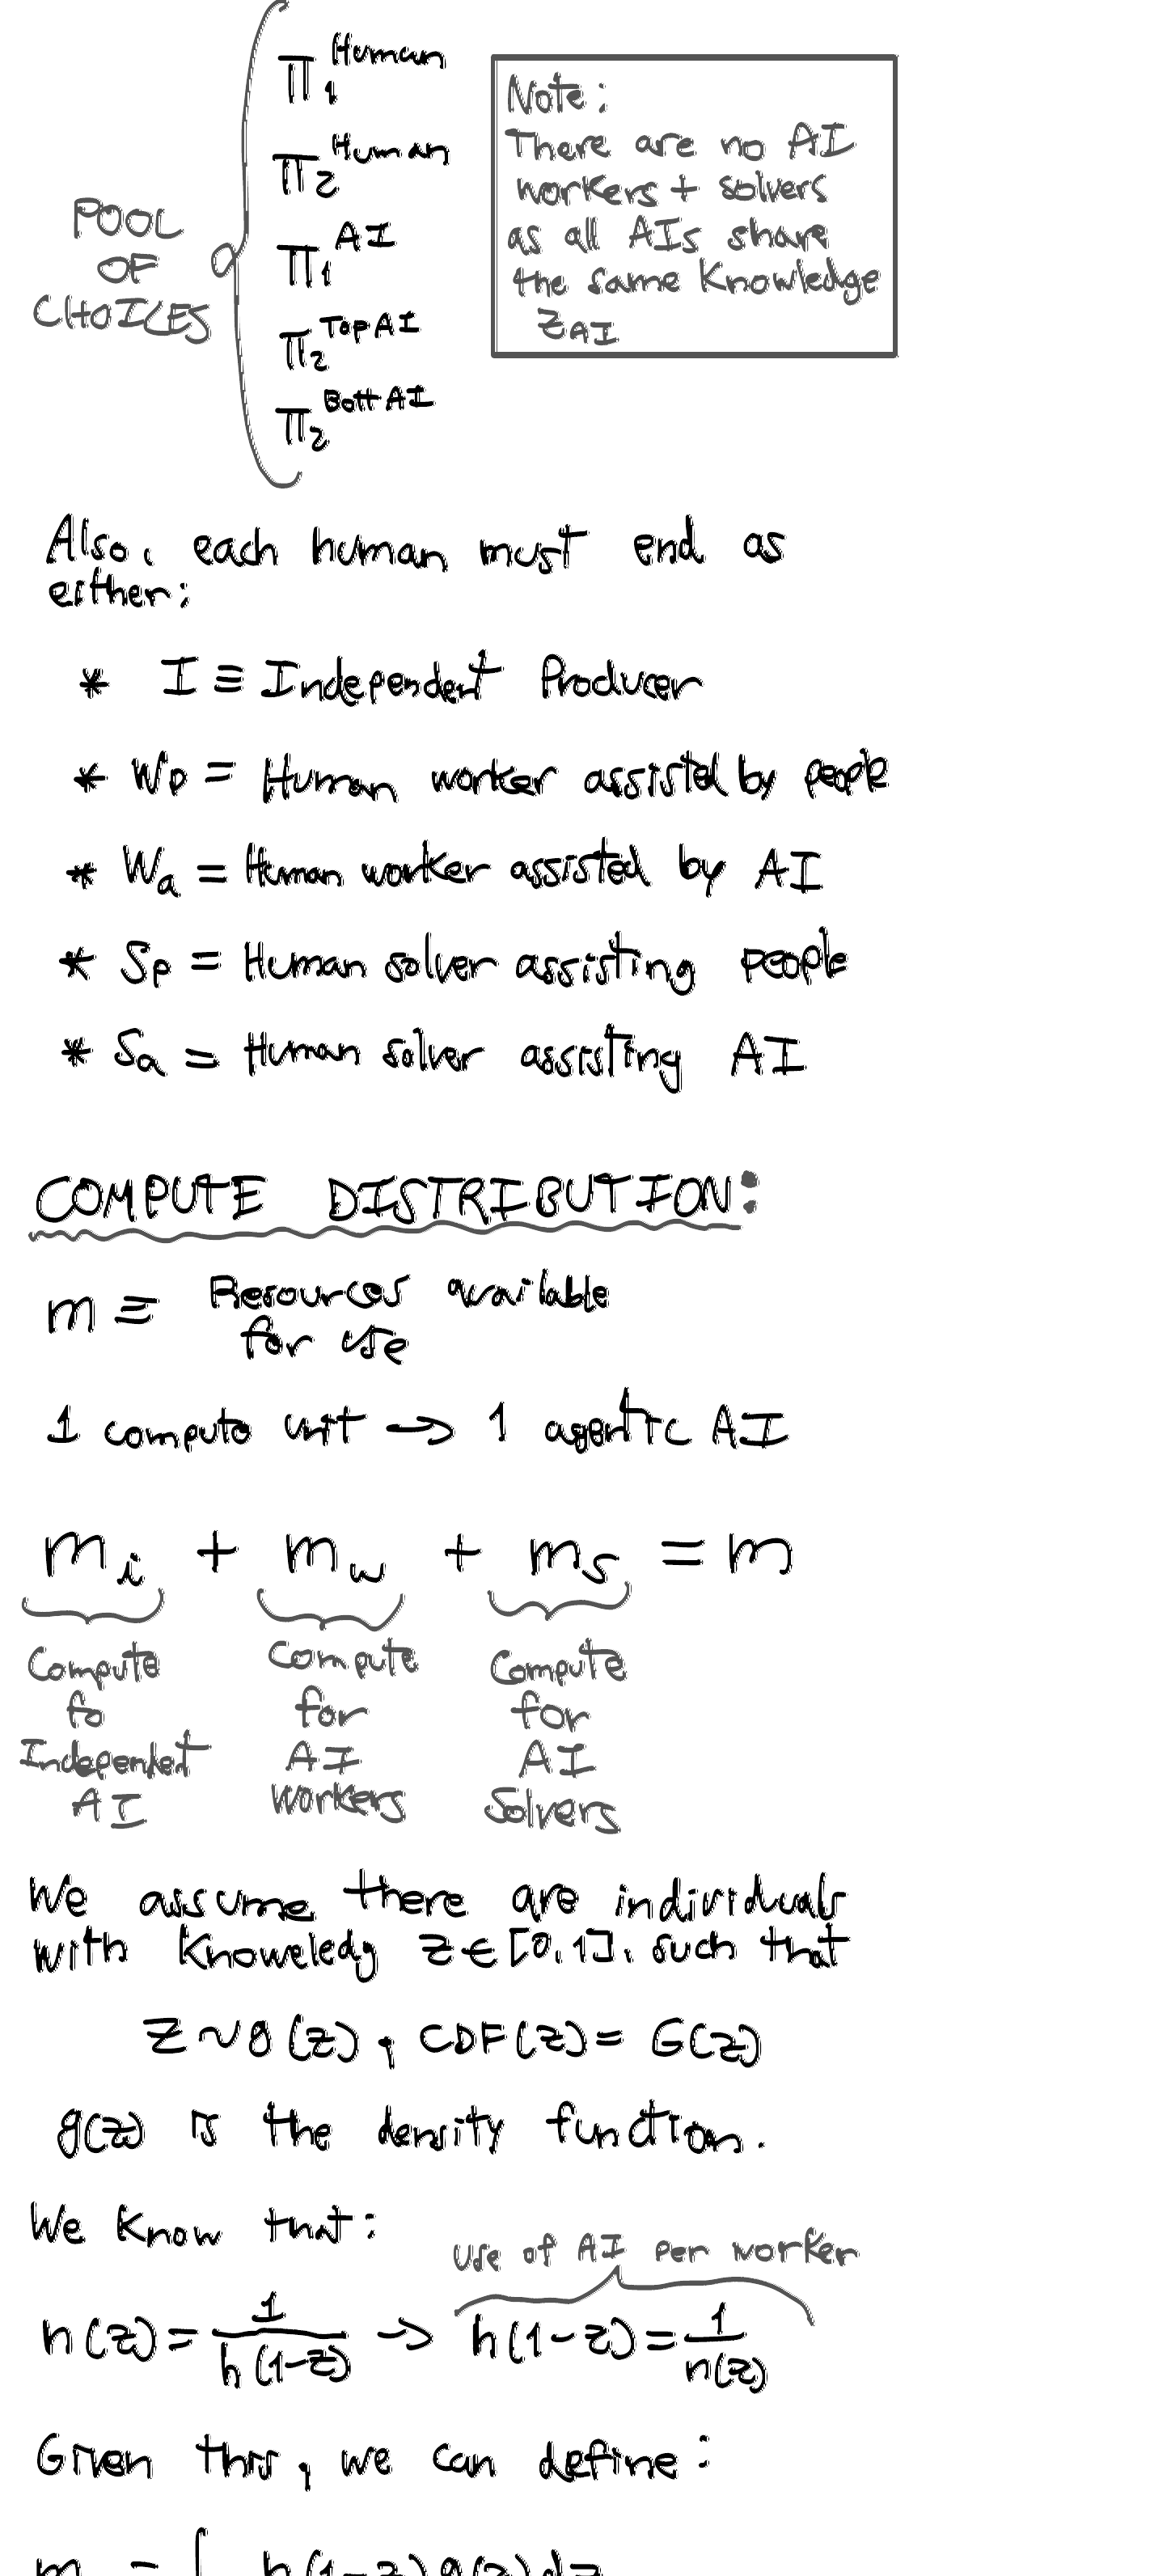
\includegraphics[height=0.84\textheight]{hand/hand-ide-talamas-2025-part4.png}\end{center}
\end{frame}
\begin{frame}{B10 \textperiodcentered{} Hand derivation 5/5: the matching condition and market clearing}
  \begin{center}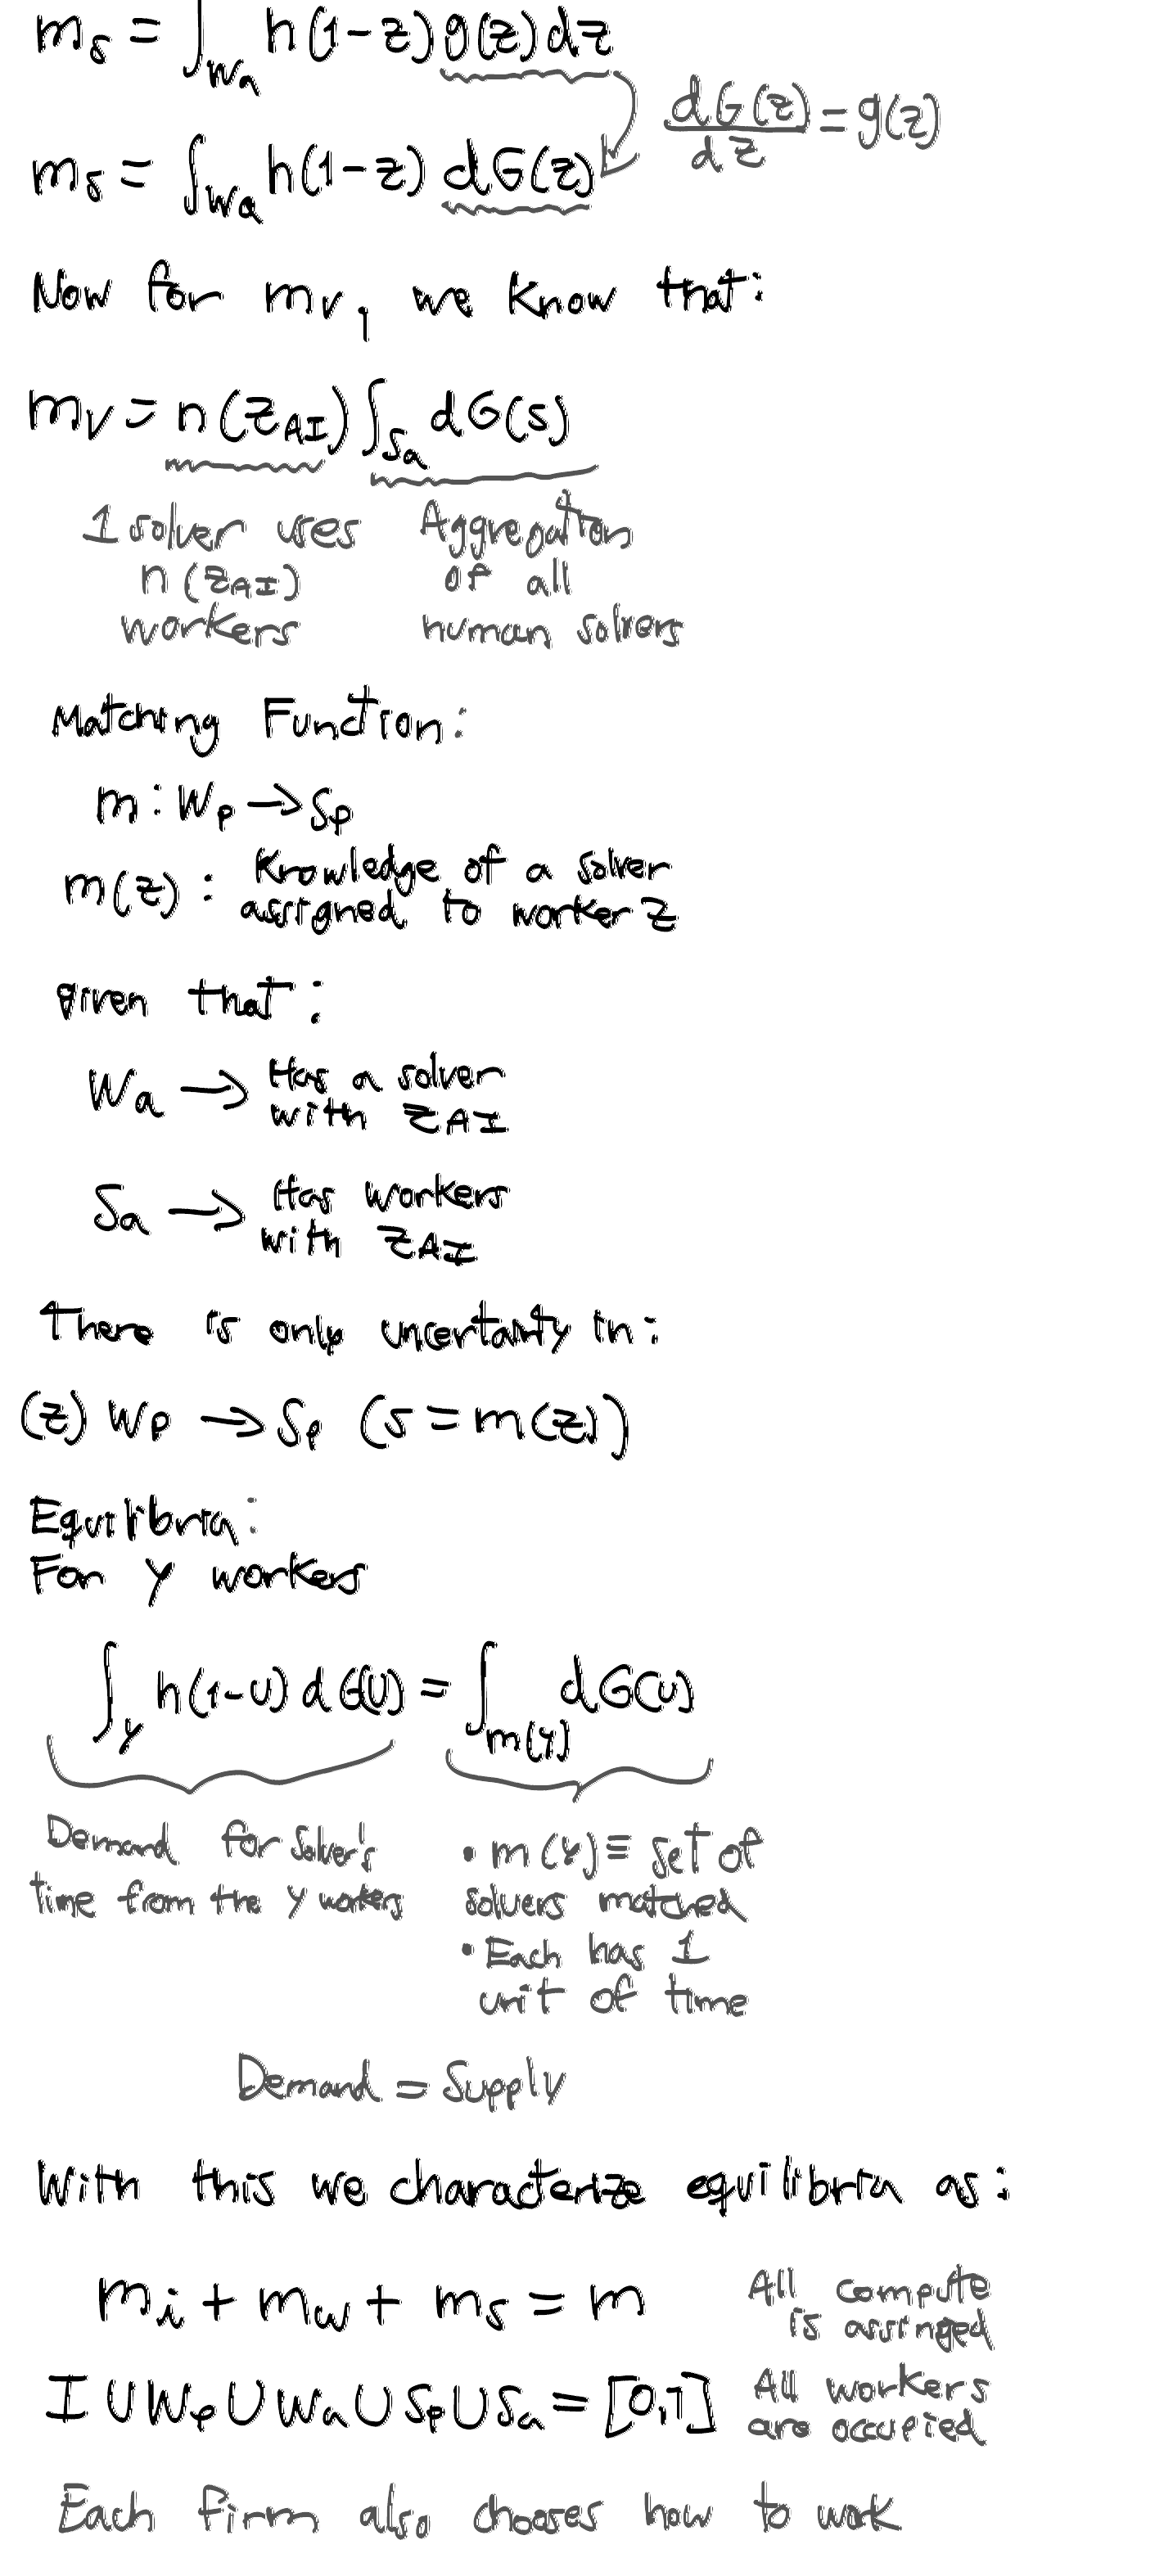
\includegraphics[height=0.84\textheight]{hand/hand-ide-talamas-2025-part5.png}\end{center}
\end{frame}

%================= BACKUP: LEAN EXTRA =================================
\begin{frame}[fragile]{B11 \textperiodcentered{} Lean IV: the span of control and Proposition 6.3}
  \scriptsize
  \begin{lstlisting}[basicstyle=\ttfamily\tiny]
def paper_span_of_controlSpec : Prop :=
  ∀ h z n : ℝ, 0 < h → h < 1 → 0 ≤ z → z < 1 →
    (h * n * (1 - z) = 1 ↔ n = 1 / (h * (1 - z)))

def paper_prop6_bottom_prefers_nonautonomousSpec : Prop :=
  ∀ h z zAI wpre : ℝ, 0 < h → h < 1 → 0 ≤ z → z < 1 → 0 < zAI →
    zAI - zAI * (1 - 1 / (1 / (h * (1 - z)))) = h * (1 - z) * zAI ∧
    zAI * (1 - 1 / (1 / (h * (1 - z)))) < zAI ∧
    (wpre < zAI ↔
      wpre < max wpre zAI ∧ zAI = max wpre zAI)

def paper_prop6_output_idle_computeSpec : Prop :=
  ∀ zAI used total Yhuman : ℝ, 0 < zAI → used < total →
    Yhuman + zAI * used < Yhuman + zAI * total
  \end{lstlisting}
  \textbf{Reading.} The first Spec is the page-10 display as an equivalence: the span of control is \emph{the} solution.
  The Prop.\ 6.3 Spec compares the three wages of a worker assisted by AI in both regimes: the non-autonomous premium
  over the autonomous wage is $z_{AI}/n(z)=h(1-z)z_{AI}$ (the AI solver's share when $r^*=z_{AI}$), and the gain over the
  pre-AI wage is exactly the condition $z_{AI}>w$ --- at $z=0$ this is the proposition's ``$z_{AI}>w(0)$''. The last
  Spec is the accounting behind 6.1: idle compute is output forgone at $z_{AI}$ per unit.
\end{frame}

\end{document}
